LSTM – là 1 dạng đặc biệt của mô hình RNN (Recurrent Neural Network), có khả năng học được các phụ thuộc. Phương pháp chính của mô hình LSTM là trạng thái tế bào (cell state), nó tương tự như 1 băng truyền chạy xuyên suốt tất cả các mắt xích và tương tác tuyến tính với các mắt xích đó vì vậy mà các thông tin dễ dàng truyền đi thông suốt mà không sợ bị thay đổi. LSTM có khả năng bỏ đi hoặc thêm vào các thông tin cần thiết cho state và được điều chỉnh thông qua các nhóm gọi là cổng (gate). Các cổng là nơi sàng lọc thông tin khi đi qua nó, chúng được kết hợp bởi một tầng mạng sigmoid và một phép nhân. Tầng sigmoid sẽ cho đầu ra là một số trong khoản [0,1] [0,1], mô tả có bao nhiêu thông tin có thể được thông qua. Khi đầu ra là 00 thì có nghĩa là không cho thông tin nào qua cả, còn khi là 11 thì có nghĩa là cho tất cả các thông tin đi qua nó. Một LSTM gồm có 3 cổng như vậy để duy trì và điều hành trạng thái của tế bào.

\begin{figure}[htbp]
\centerline{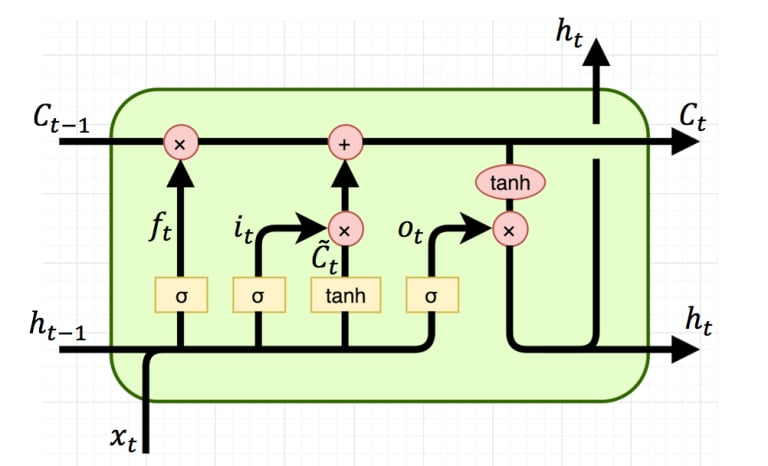
\includegraphics[width=0.4\textwidth]{img/LSTM.jpg}}
\caption{Kiến trúc LMST.}
\label{fig}
\end{figure}